\chapter{Spectrometer Alignment} \label{ch::alignment}
\ifpdf
\graphicspath{{Chapters/Alignment/Figs/Raster/}{Chapters/Alignment/Figs/PDF/}{Chapters/Alignment/Figs/}}
\else \graphicspath{{Chapters/Alignment/Figs/Vector/}{Chapters/Alignment/Figs/}}
\fi

The alignment of the spectrometer is important for track reconstruction.
Alignment is a part of pre-processing which ensures all the tracking detectors
are centered relative to each other and therefore enables the track resolution
to be as accurate as possible.  Without accurate alignment, track reconstruction
is not possible and it is therefore not possible to analyze any data.  The
author of this thesis oversaw collection of alignment data and was
responsible for performing the alignment of the COMPASS spectrometer in 2015.

The objective of the alignment procedure is to produce a file called the
detectors.dat.  This file describes the parameters for all detectors at COMPASS
and in particular, gives their orientation in space.  For a tracking detector
plane, there are four parameters the alignment procedure updates: the x central
position, y central position, angle and the pitch.  The pitch refers to a sense
wire distance for wire chambers or central strip separation distance for
detectors with strip readouts.  One or two detectors.dat files was produced for
each data taking period, depending on how many alignment runs were recorded that
period.  The goal of the alignment procedure is to have all four parameters
aligned relative to a global reference frame in the COMPASS lab system.

The alignment procedure works by minimizing the distance between all the
detector plane hit positions and a track position.  The detector hit position is
the location the detector believes a particle passed through the plane and the
track position is the location the reconstruction believes the particle passed
through the detector plane.  The distance between this detector plane hit
position and the track position will from here on be referred to as the residual
distance.  One residual is determined per track per detector associated with the
track.  The task of simultaneously minimizing all the residuals is difficult
because there are over 300 detectors planes described in the detectors.dat.  To
accomplish this minimization, a large amount of quality data is needed and
several specific matrix manipulations are utilized in the minimization
procedure.  This chapters gives an overview of the alignment procedure and
includes some results from 2015.  For a more complete review see
reference~\cite{compassAlignmentNote}.


\section{Alignment Data}

The alignment data is produced from a dedicated low intensity muon beam.  The
intensity in 2015 was approximately 10$^5 \mu^-$/spill.  A muon beam is
desirable for alignment data because the beam muons interact less and therefore
allows the alignment procedure to assume straight tracks in the minimization
problem.  The lower intensity is chosen because this allows for the assumption
that only one track occurs per event and also the low intensity beam ensures a
reduction of detector pile up effects.  Reduction in pile up effects, makes
reconstruction in the central detector areas possible, and therefore the beam
killers on DC00, DC01, DC04 and DC05 can be set to an amplification voltage and
as well all the GEM detectors can have their central high voltages turned up to
an amplification voltage.

A dedicated trigger system is setup during alignment runs to maximize the
illumination of the tracking detectors.  The triggers used are a beam trigger,
veto trigger and a halo trigger.  While this trigger was good for illuminating
the detectors, there were some timing shifts relative to the normal Drell-Yan
trigger in 2015.  For this reason some of the drift chambers used a different
calibration curve shifted in time a few nanoseconds.

Two alignment runs of good quality are recorded either at the beginning, middle
or end of a data taking period.  The first alignment run is with the
spectrometer magnets off and the second is with the spectrometer magnets on.
The spectrometer magnets off run is used as a first iteration for the alignment
procedure to initialize the tracking detector positions.  The final alignment
positions are then determined from the spectrometer magnets on data.  

One physics run was also used to align detectors far from the beam line.
Particularly, the outer region of the straw detectors did not receive enough
statistics from the aligning runs.  Therefore the alignment of the outer straw
regions was performed with normal physics data.  The runs used for alignment
analysis in 2015 are listed in Table~\ref{tab::alignmentRuns}.

In 2015 the alignment runs were performed when the target solenoid was
polarizing the target.  The chicane magnets upstream of the target were
therefore turned off to ensure the beam momentum was traveling along the target
axis.  Normally to achieve the reduced intensity, the T6 target is switch to an
air target.  However in 2015, the T6 target head was not able to switch between
the different target lengths and therefore the maximum 500~mm target head was
always in use.  Therefore to achieve the desired lower intensity, a set of
collimeters upstream of the target reduced the aperture of the beam line till
the correct intensity was achieved.

\begin{table}[h!t]
  \centering
  \begin{tabular}{ |c|c|c|c|c|c| }
    \hline
    \textbf{Period}& \textbf{Sub-period}& \textbf{Magnets off run}&
    \textbf{Magnets on run}& \textbf{Physics run}&
    \textbf{detectors.dat name} \\ \hline
    
    W07& one \& two & 259360& 259361& 259363& detectors.259361.transv.dat
    \\ \hline

    W08& one \& two & 260072& 260073& 260100& detectors.260073.transv.dat
    \\ \hline

    \multirow{2}{2em}{W09}& one& 260625& 260626& 260661&
    detectors.260626.transv.dat \\
    & two& 260625& 260876& 261312&
    detectors.260876.transv.dat \\ \hline

    \multirow{2}{2em}{W10}& one& 261512& 261513& 261602&
    detectors.261513.transv.dat \\
    & two& 261512& 261513& 261974&
    detectors.261970.transv.dat \\ \hline

    W11& one \& two & 262423& 262425& 262612& detectors.262370.transv.dat
    \\ \hline

    W12& one \& two & 263139& 263140& 263175& detectors.263140.transv.dat
    \\ \hline

    W13& one \& two & 263636& 263637& 263851& detectors.263637.transv.dat
    \\ \hline

    W14& one \& two & none& 264428& 264429& detectors.264163.transv.dat
    \\ \hline

    W15& one \& two & 264614& 264722& 264736& detectors.264619.transv.dat
    \\ \hline
    
  \end{tabular}
  \caption{COMPASS 2015 alignment data runs}
  \label{tab::alignmentRuns}
\end{table}


\section{Procedure}

The starting point for alignment is a detectors.dat file with the tracking
detector positions determined from a survey.  The surveys are performed with the
spectrometer magnets off and the precision from a survey is around 1~mm.  Almost
all of the detectors at COMPASS have a position resolution better than the
survey precision however.  Furthermore, several detectors near SM1 can shift in
position due to the fringe field and therefore need a position determination
with the spectrometer magnets on.  For these reasons the alignment procedure is
needed to improve on the survey precision and achieve the best possible track
resolutions.

Between periods the starting detectors.dat file was the final detectors.dat from
the previous week.  Only for the first period were the survey positions used as
a starting position.  However, as long as the detector was not intentionally
moved, it is expected that the shifts in detector position only change due to
temperature effects and therefore do not change much.

\subsubsection{Alignment Parameters}

To best describe each detector relative to every other detector there are two
reference systems of interest.

The first reference system is the COMPASS main reference system labeled
\textit{Oxyz}.  This reference system can also be referred to as the COMPASS lab
system, where the z-axis is along the beam momentum direction, the y-axis points
vertically and the x-axis is such that the coordinate system is right handed.
The origin of this reference system is at the center of the target from the
original COMPASS setup.

The second reference system is the local reference system, which is labeled as
\textit{O'uvz}.  This reference system is different for each detector and has
its origin at the center of each detector center.  The z-axis coincides with the
z-axis in the COMPASS main reference system while the u-axis is in the direction
along the measured coordinate of the detector, and the v-axis is perpendicular to
the direction of the measured coordinate of this detector.  As an example, a drift
chamber with vertical wires measures a coordinate along the horizontal direction
and therefore it's u-axis is in the horizontal direction and it's v-axis is in
the vertical direction.  A drift chamber with horizontal wires, however,
measures a coordinate along the vertical direction and therefore it's u-axis is
in the vertical direction and it's v-axis is in the horizontal direction.

The alignment parameters are defined in \textit{O'uvz}.  The alignment procedure
updates the starting detectors.dat file by the shifts

\begin{align}
  \delta \mathrm{u} & \mathrm{: \; shift \; in \; u \; direction,}  \\
  \delta \theta & \mathrm{: \; shift \; in \; rotation \; angle,}  \\
  \delta \mathrm{z} & \mathrm{: \; shift \; in \; z \; direction,}  \\
  \delta \mathrm{p} & \mathrm{: \; shift \; in \; pitch.} 
\end{align}
\noindent
The shift in z direction has never converged however.  As a result the
z-coordinate from the survey is used as the final z position and the shift in
pitch is used as an effective shift in the z direction.

\subsubsection{Residual Function}

The goal of the alignment procedure is to minimize the sum of all the residuals
from each track and each detector associated with the track.  Due to the fact
that the alignment tracks are assumed to be straight, each track can be defined
by four parameters.  The track parameters, {\atrack}, are

\begin{enumerate}[label=\roman*:]
\item (x$^0$, y$^0$) the x and y coordinates at the main reference origin
\item (t$_{\mathrm{x}}^0$, t$_{\mathrm{y}}^0$) the tangents of the track
  momentum in the x and y directions at the origin of the main reference system
\end{enumerate}
\noindent
where the track parameters are defined for each track.  The alignment parameters
, {\adet}, on the other hand are defined for each detector and are the same for
all tracks.  The alignment procedure minimizes the $\chi^2$ function

\begin{equation}
  \chi^2 =
  \sum_{i=1}^{i=n_{\mathrm{tracks}}}\sum_{j=1}^{j=n_{\mathrm{detectors}}}
  \frac{\mathrm{F}^2_{i,j}(\alpha_{\mathrm{T}, i}, \alpha_{\mathrm{D},
      j})}{\sigma_j^2},
  \label{equ::chi_align}%
\end{equation}
\noindent
where $\sigma^2_j$ is the position resolution of detector j, F$_{i,j}$ is the
residual distance of each detector j for each track i it is associated with.

The residual distance, F, depends on the track parameters and the detector
parameters.  For magnets off data the tracks are not bent at all and are
therefore straight tracks through out the whole spectrometer.  The x and y coordinates at position z are

\begin{align}
  \label{equ::trackPosOff}
  \mathrm{x} &= \mathrm{x}^0 +
  \mathrm{t}_{\mathrm{x}}^0(\mathrm{z}-\mathrm{z}^0), \\
  \mathrm{y} &=
  \mathrm{y}^0 + \mathrm{t}_{\mathrm{y}}^0(\mathrm{z}-\mathrm{z}^0),
\end{align}
\noindent
where z$^0$ refers to the position at the origin in \textit{Oxyz}.
Rotating these track positions from the main references system, \textit{Oxyz},
to the detector reference system, \textit{O'uvz}, the residual distance is

\begin{equation}
\mathrm{F} = \cos(\theta)[\mathrm{x}^0 +
  \mathrm{t}_{\mathrm{x}}^0(\mathrm{z}-\mathrm{z}^0)] +
\sin(\theta)[\mathrm{y}^0 + \mathrm{t}_{\mathrm{y}}^0(\mathrm{z}-\mathrm{z}^0)]
- \mathrm{u},
\end{equation}
\noindent
where u is the measured hit position from the detector at position z.  To show
the dependence on the alignment parameters

\begin{dmath} \label{equ::Falign}
  \mathrm{F}(\alpha_{\mathrm{T}}, \alpha_{\mathrm{D}}+\delta\alpha_{\mathrm{D}})
  = (1+\delta \mathrm{p})
  \Big \{ \cos(\theta + \delta \theta)
       [\mathrm{x}^0 + \mathrm{t}^0_{\mathrm{x}}(\mathrm{z}-\mathrm{z}^0)] +
       \sin(\theta + \delta \theta)[\mathrm{y}^0 + \mathrm{t}^0_{\mathrm{y}}
         (\mathrm{z}-\mathrm{z}^0)] \Big \} -
       (\mathrm{u} + \delta \mathrm{u}).
\end{dmath}
\noindent
In Eq.~\ref{equ::Falign}, the change in pitch would intuitively affect the u
position, however the change in pitch was moved to the track coordinates to make
derivatives of F independent of u.  This has no effect on the minimization of F.

In the case of magnets on data, the track positions need to have further
modifications from Eq.~\ref{equ::Falign}.  The magnetic field will bend the
tracks so the track positions determined in Eq.~\ref{equ::trackPosOff} need to
have further corrections.  The track positions with SM1 and SM2 on are
\begin{align}
  \label{equ::trackPosOn}
  \mathrm{x} &= \mathrm{x}^0 + \delta\mathrm{x} +
  (\mathrm{t}_{\mathrm{x}}^0 + \delta \mathrm{t}_{\mathrm{x}})
  (\mathrm{z}-\mathrm{z}^0), \\
  \mathrm{y} &= \mathrm{y}^0 + \delta\mathrm{y} +
  (\mathrm{t}_{\mathrm{y}}^0 + \delta \mathrm{t}_{\mathrm{y}})
  (\mathrm{z}-\mathrm{z}^0),
\end{align}
\noindent
where the $\delta_{\mathrm{x}}$, $\delta \mathrm{t}_{\mathrm{x}}$,
$\delta_{\mathrm{y}}$ and $\delta \mathrm{t}_{\mathrm{y}}$ changes are
determined from CORAL during the reconstruction process.  Even though the
spectrometer magnets have nominally vertical magnetic fields, there are still
fringe fields which are not vertical.  It is for this reason that CORAL also
calculates an updated track position in the y-coordinate.

The residual dependence on the alignment parameters defined for magnetic fields
on is then
\begin{dmath}
  \mathrm{F}(\alpha_{\mathrm{T}},
  \alpha_{\mathrm{D}}+\delta\alpha_{\mathrm{D}}) = 
  (1+\delta \mathrm{p})\Big \{
\cos(\theta + \delta \theta)[\mathrm{x}^0 + \delta\mathrm{x} +
  (\mathrm{t}^0_{\mathrm{x}}+\delta \mathrm{t}_{\mathrm{x}})
  (\mathrm{z}-\mathrm{z}^0)] +
\sin(\theta + \delta\theta)[\mathrm{y}^0 + \delta\mathrm{y} +
  (\mathrm{t}^0_{\mathrm{y}}+\delta \mathrm{t}_{\mathrm{y}})
  (\mathrm{z}-\mathrm{z}^0)]
\Big \}
- (\mathrm{u} + \delta \mathrm{u}).
\end{dmath}

\subsubsection{$\chi^2$ Minimization}
The $\chi^2$ function, Eq.~\ref{equ::chi_align}, is analytically minimized.
That is, the derivatives of Eq.~\ref{equ::chi_align} with respect to all the
track and alignment parameters are set to zero and these alignment parameters
are solved for.  This can be written

\begin{equation}
  \label{equ::chi2analytic}
  \frac{1}{2}\frac{\partial \chi ^2}{\partial \alpha_k} =
  \sum_{i}^{n_{\mathrm{tracks}}} \sum_j ^{n_{\mathrm{detectors}}}
  \frac{1}{\sigma_j^2}\frac{\partial \mathrm{F}_{i,j}}{\partial \alpha_k}
  \mathrm{F}_{i,j} = 0.
\end{equation}

\noindent
To perform this calculation the residual function is Taylor expanded in the
track and alignment parameters as
\begin{equation}
\mathrm{F} = \mathrm{F}^0 + \sum_k \frac{\partial \mathrm{F}}{\partial
  \alpha_k}\alpha_k.
\end{equation}

\noindent
Using this approximation for F, Eq.~\ref{equ::chi2analytic} can be written as a
matrix equation where the dimensions of the matrix are
(4n$_{\mathrm{detector}}$+4n$_{\mathrm{tracks}})\times$
(4n$_{\mathrm{detector}}$ +4n$_{\mathrm{tracks}})$.  This matrix form is written
as

\begin{dmath}
  \begin{bmatrix}
    \sum_i^{n_{\mathrm{tracks}}} \sum_j^{n_{\mathrm{detectors}}}
      \frac{1}{\sigma^2_j} \frac{\partial \mathrm{F}_{i,j}}{\partial
        \alpha_{\mathrm{D_1}}}\frac{\partial \mathrm{F}_{i,j}}{\partial
        \alpha_{\mathrm{D_1}}}
      & \dots &
      \sum_j^{n_{\mathrm{detectors}}}
      \frac{1}{\sigma^2_j}\frac{\partial \mathrm{F}_{i,j}}{\partial
        \alpha_{\mathrm{D_1}}}\frac{\partial \mathrm{F}_{i,j}}{\partial
        \alpha_{\mathrm{T_{4\mathrm{n}_{\mathrm{tracks}}}}}} \\
      \vdots & \ddots & \vdots \\
      \sum_j^{n_{\mathrm{detectors}}}
      \frac{1}{\sigma^2_j}\frac{\partial \mathrm{F}_{i,j}}{\partial
        \alpha_{\mathrm{T_{4\mathrm{n}_{\mathrm{tracks}}}}}}\frac{\partial
        \mathrm{F}_{i,j}}{\partial \alpha_{\mathrm{D_1}}} & \dots &
      \sum_j^{n_{\mathrm{detectors}}} \frac{1}{\sigma^2_j}\frac{\partial
        \mathrm{F}_{i,j}}{\partial
        \alpha_{\mathrm{T_{4\mathrm{n}_{\mathrm{tracks}}}}}}\frac{\partial
        \mathrm{F}_{i,j}}{\partial
        \alpha_{\mathrm{T_{4\mathrm{n}_{\mathrm{tracks}}}}}}
  \end{bmatrix}
  \begin{bmatrix}
    \alpha_{\mathrm{D_1}} \\
    \vdots \\
    \alpha_{\mathrm{T_{4\mathrm{n}_{\mathrm{tracks}}}}}
  \end{bmatrix}
  = -
  \begin{bmatrix}
    \sum_i^{n_{\mathrm{tracks}}} \sum_j^{n_{\mathrm{detectors}}}
      \frac{1}{\sigma^2_j}\frac{\partial \mathrm{F}_{i,j}}{\partial
        \alpha_{\mathrm{D_1}}} \mathrm{F}_{i,j}^0 \\
      \vdots \\
      \sum_j^{n_{\mathrm{detectors}}}
    \frac{1}{\sigma^2_j}\frac{\partial \mathrm{F}_{i,j}}{\partial
      \alpha_{\mathrm{T_{4\mathrm{n}_{\mathrm{tracks}}}}}} \mathrm{F}_{i,j}^0
  \end{bmatrix}.
  \label{equ::aliMatrix}
\end{dmath}    

\noindent
To solve Eq.~\ref{equ::aliMatrix}, the matrix on the left side must be inverted.
A normal alignment run however, results in over 200,000 tracks meaning this
matrix is huge and infeasible to invert.  Fortunately many of the entries in the
matrix are zero which allows that this matrix inversion can be reduced to
the inversion of several smaller matrices.

To perform the matrix inversion, note that Eq.~\ref{equ::aliMatrix} can be
written

\begin{equation}
  \label{equ::matrixToInvert}
  \begin{bmatrix}
    \sum_{i} \mathrm{C}_i & \vline \; \vline \; & \dots &
    \mathrm{G}_i & \dots \\
    \hline \hline
    \vdots & \vline \; \vline & \ddots & 0 & 0 \\
    \mathrm{G}^{\mathrm{T}} & \vline \; \vline & 0 \; & \Gamma_i & 0 \\
    \vdots & \vline \; \vline & 0 & 0 & \ddots
  \end{bmatrix}
  \begin{bmatrix}
    \alpha_{\alpha} \\ \hline \hline \vdots \\ \alpha_{\mathrm{T}_i}
    \\ \vdots
  \end{bmatrix}
  =
  \begin{bmatrix}
    \sum_i b_i \\ \hline \hline \vdots \\ \beta_i \\ \vdots
  \end{bmatrix},
\end{equation}

\noindent
where $\sum_i$C$_i$ and $\sum_i$b$_i$ include only derivatives of F$_{i,j}$ with
respect to alignment parameters, $\Gamma_i$ and $\beta_i$ include only
derivatives of F$_{i,j}$ with respect to track parameters and G$_i$ includes
derivatives of F$_{i,j}$ with respect to both alignment and track parameters.
Then reference~\cite{matrix_inv} shows that Eq.~\ref{equ::matrixToInvert} can be
inverted to give the alignment parameters as

\begin{equation}
\alpha_{\alpha} = \mathrm{C'}^{-1}\mathrm{b}',
\end{equation}
\noindent
where
\begin{equation}
\mathrm{C}' = \sum_i \mathrm{C}_i - \sum_i \mathrm{G}_i \Gamma_i^{-1}
\mathrm{G}_i^{\mathrm{T}},
\end{equation}
\noindent
and
\begin{equation}
\mathrm{b}' = \sum_i \mathrm{b}_i - \sum_i \mathrm{G}_i \Gamma_i^{-1}\beta_i.
\end{equation}


\section{Results}

The spectrometer alignment is performed in iterative steps.  In each iteration
of the alignment procedure, the matrix inversion, Eq~\ref{equ::matrixToInvert},
is performed and the alignment parameters are updated.  All alignment tracks
reconstructed in the first alignment iterations are based off of two pivot
detectors.  That is straight track parameters were determined from these two
pivot detectors and all detectors were aligned relative to these pivot
detectors.  In 2015 the pivot detectors were GM05 in LAS and GM08 in SAS.  After
each iteration the detector parameters are updated to reduce the overall
$\chi^2$ value.  Each new iteration is performed using the same data set and the
alignment parameters are better described with each iteration.

The procedure used in 2015 was as follows:
\begin{enumerate}
\item Align with magnets off data.  In this stage all the spectrometer detectors
  except the outer regions of the straw detectors are aligned.  This includes
  all the detectors downstream of the polarized target but does not include the
  beam telescope detectors.  Magnets off data is used as a first iteration and
  therefore only alignment in the u-coordinate is performed.
\item Align the same spectrometer detectors with magnets on data.  In these
  iterations the detectors are aligned for u-coordinate, angle and pitch.
\item Align the beam telescope detectors with magnets on data.  In these
  iterations the previous detectors are all used as pivots.  The beam telescope
  is therefore aligned relative to the spectrometer detectors.
\item Finally the outer region of the straws are aligned with physics data.  For
  this alignment, the spectrometer detectors are again used as the pivot.
\end{enumerate}

The quality of the alignment was monitored after each iteration and checked that
the procedure was converging.  In practice four iterations of each of the
previous steps were found to be sufficient for convergence.  To ensure the
alignment data was from quality tracks, only tracks with momentum reconstructed
and having reduced $\chi^2$ less than 30 were considered.

As all detectors but the pixal detector planes measure a coordinate in one
direction only, the detector positions are only updated in their measured
direction.  This can lead to detectors being well miss-aligned in the direction
orthogonal to their measured coordinate however.  To account for this, detector
planes were updated to match the u-position from a detector plane measuring a
different coordinate in the same detector station.  For example DC04X planes had
their y-coordinate determined from the DC04Y planes and DC04Y planes had their
x-coordinate determined from DC04X planes.

After each alignment iteration the quality of the alignment is accessed for each
individual detectors and for the spectrometer as a whole.  The quality
distributions to check after each iteration are described in the following list.

\begin{enumerate}[label=\roman*)]
\item The residual distribution, $\Delta$u, of each detector.  That is a
  distribution of
  \begin{equation}
    \Delta \mathrm{u} =
    \mathrm{u}_{\mathrm{track}} - \mathrm{u}_{\mathrm{detector}},
  \end{equation}
  where this distribution indicates if the detector is shifted along the
  direction of its measured coordinate.  This distribution is expected to be a
  Gaussian with a zero mean and an RMS value comparable to the position
  resolution of the detector.  Any deviation from a zero mean indicates the
  detector is shifted and a large RMS value indicates the detector is not
  performing as expected.  It the detector is not performing as expected the
  most obvious reason is the calibrations used for that detector are not
  accurate.  Fig.~\ref{fig::PositionResidual} shows an example of this
  distribution to monitor.
  \begin{figure}[h!t]
  \centering 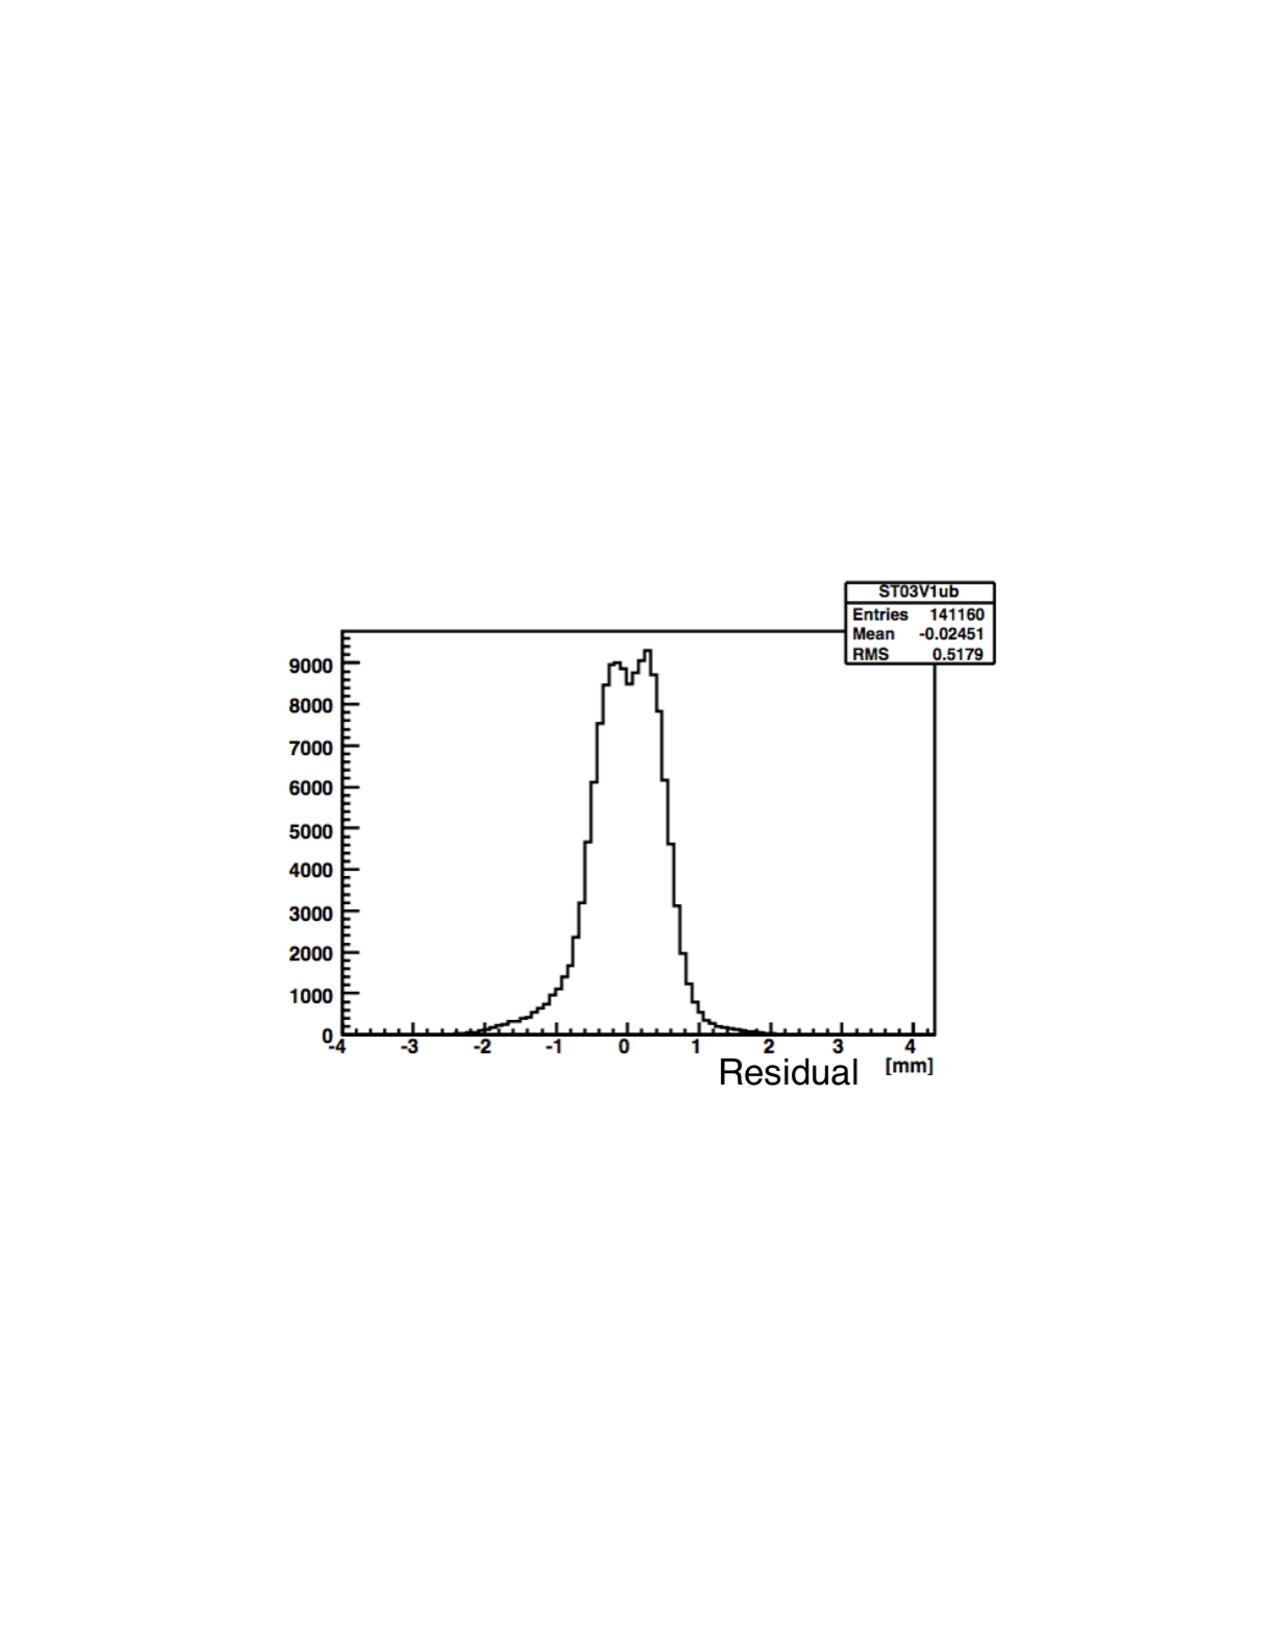
\includegraphics[width=0.5\textwidth, trim=4.5cm 9.5cm 4.5cm 9cm,
    clip]{PositionResidual}
  \caption{The residual distribution for a straw detector plane}
  \label{fig::PositionResidual}
  
\end{figure}
\item The change in the residual as a function of the detector's v-coordinate.
  In a wire detector for example, this is the change in the residual as a
  function of the distance along the wire.  This distribution,
  Fig.~\ref{fig::AngleResidual}, is expected to be uniformly zero.  A slope in
  this distribution indicates that the detector's angle is miss-aligned.
  \begin{figure}[h!t]
    \centering 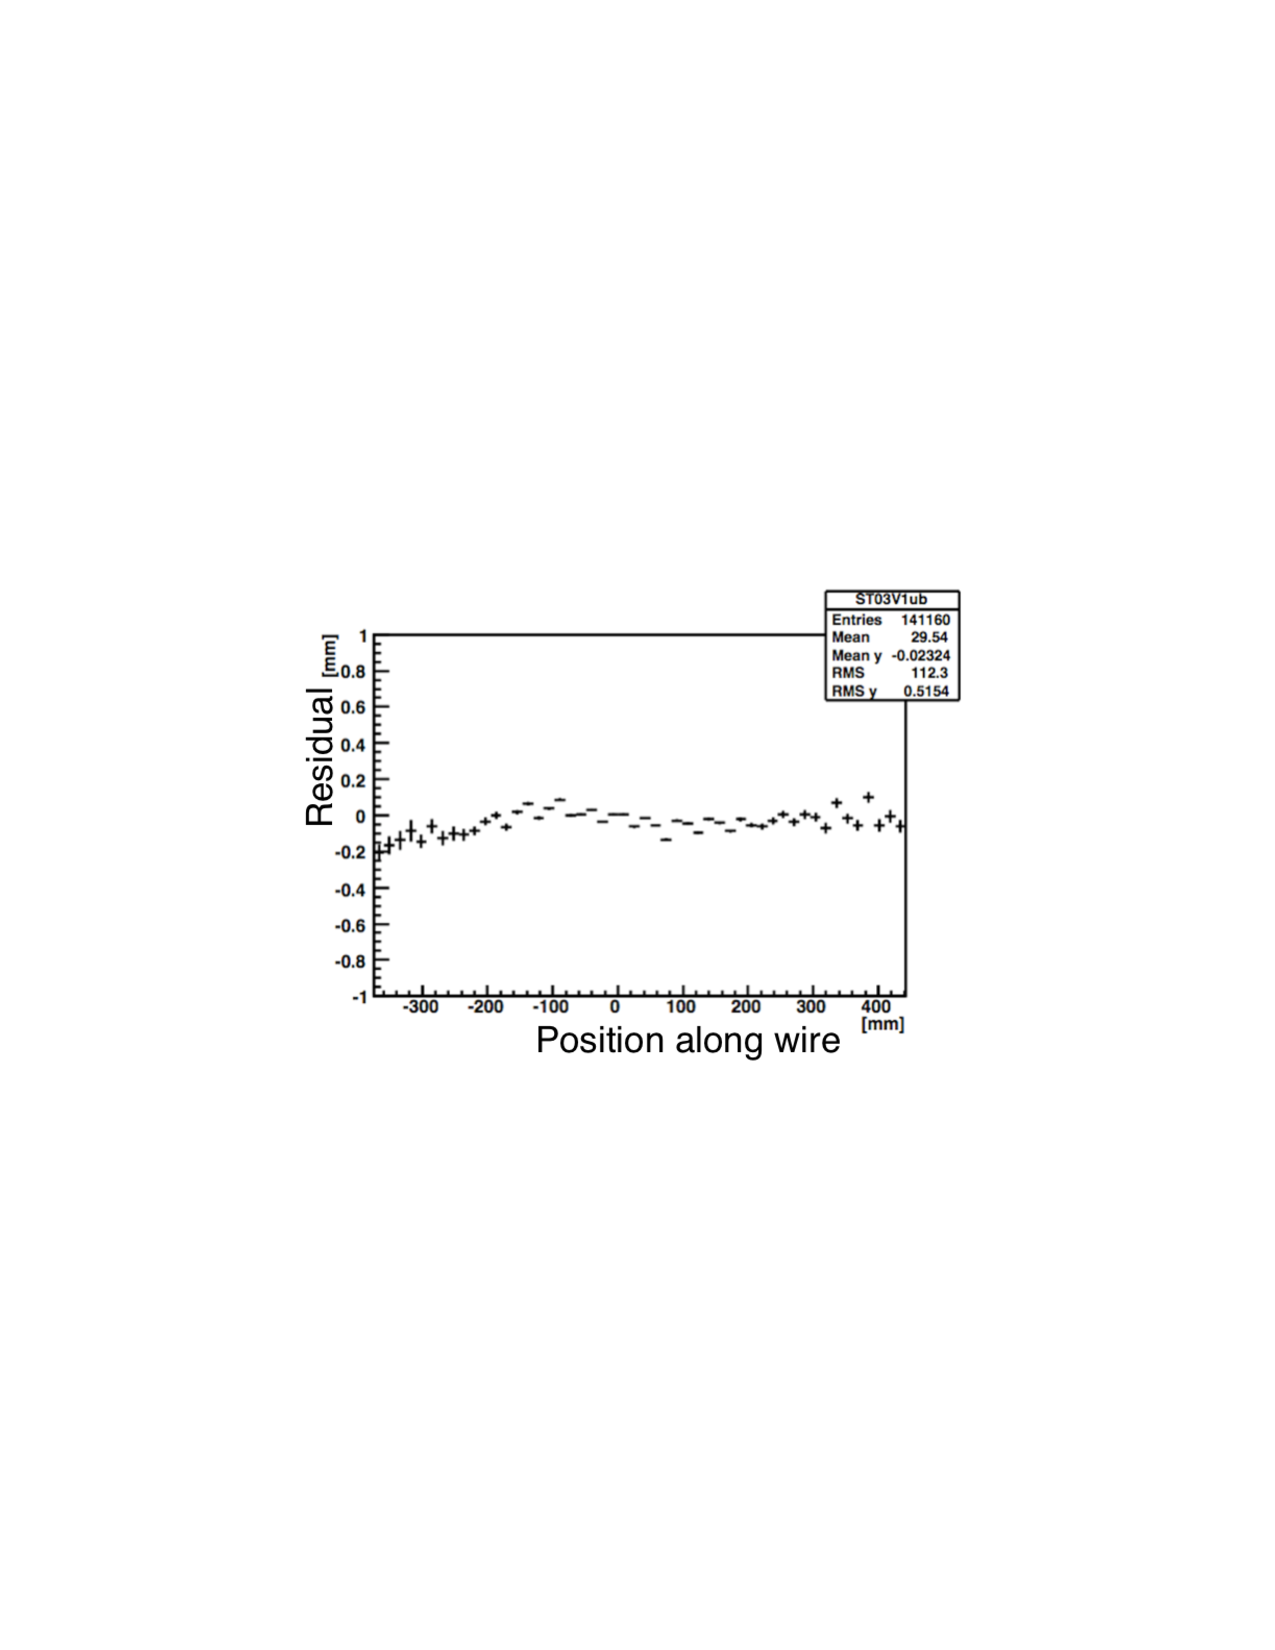
\includegraphics[width=0.5\textwidth, trim=4.5cm 9.5cm 4.5cm 9cm,
      clip]{AngleResidual}
    \caption{The residual as a function of the detector v-coordinate for a straw
      detector}
    \label{fig::AngleResidual}
  \end{figure}
  
\item The change in the residual as a function of the detector's u-coordinate.
  For a wire detector, this is the change in the residual as a function of the
  distance perpendicular to the wire.  This distribution,
  Fig.~\ref{fig::PitchResidual}, is also expected to be uniformly zero.  A slope
  in this distribution indicates that the detector is miss-aligned in it's
  z-coordinate or that its pitch is not described well.  Due to the fact that
  the alignment data is with straight tracks, the alignment in the z-coordinate
  has never been able to converge.  For this reason the pitch of the sensors on
  the detector is changed to account for this effective shift in z-position.
  The sensor pitch however, is never expected to be larger than the true
  detector pitch distance.  If the detector pitch is determined to be too large
  after the alignment, this indicates a problem.
  \begin{figure}[h!t]
    \centering 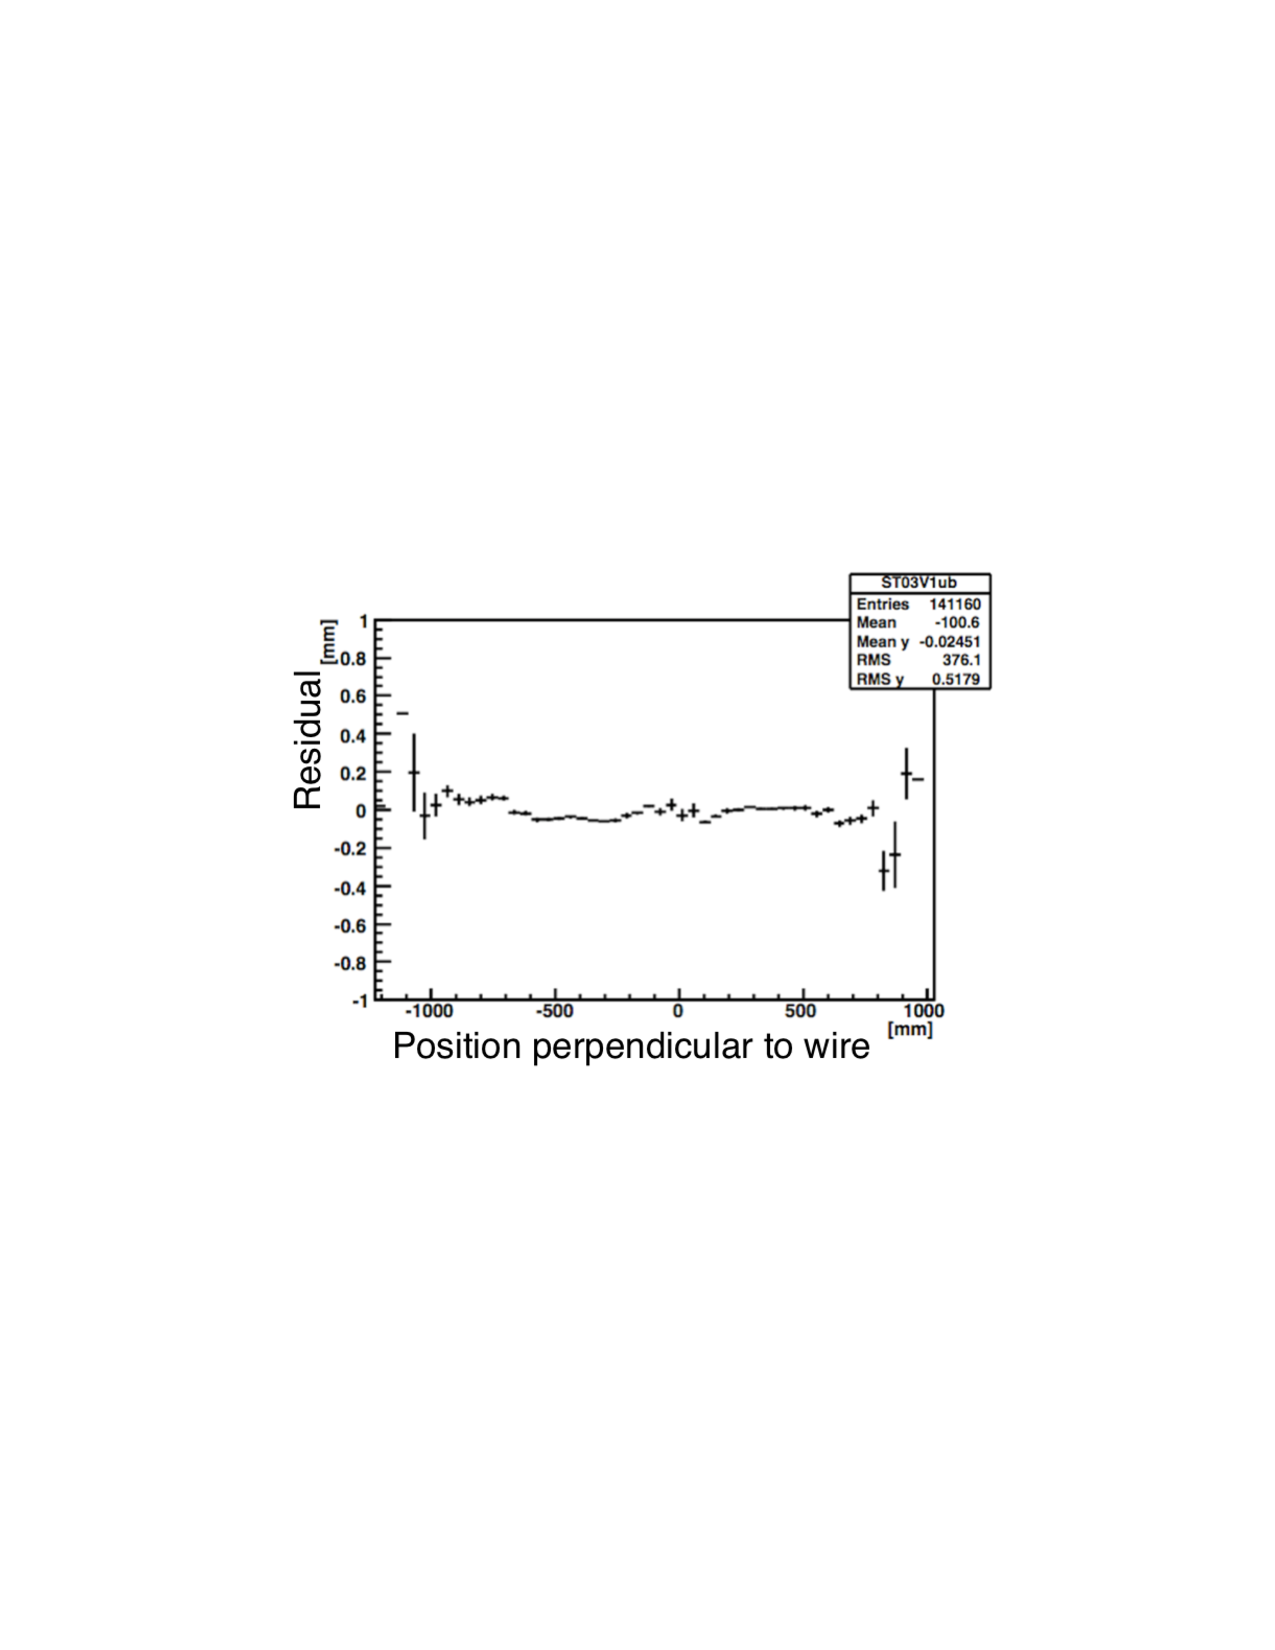
\includegraphics[width=0.5\textwidth, trim=4.5cm 9.5cm 4.5cm 9cm,
      clip]{PitchResidual}
    \caption{The residual as a function of the detector u-coordinate for a straw
      detector}
    \label{fig::PitchResidual}
  \end{figure}

\item The reduced $\chi^2$, Fig.~\ref{fig::trackChi2ndf}, distribution of the
  reconstructed tracks.  With better alignment the track reduced $\chi^2$
  distribution will approach a theoretical distribution of a reduced $\chi^2$
  distribution.
  \begin{figure}[h!t]
    \centering 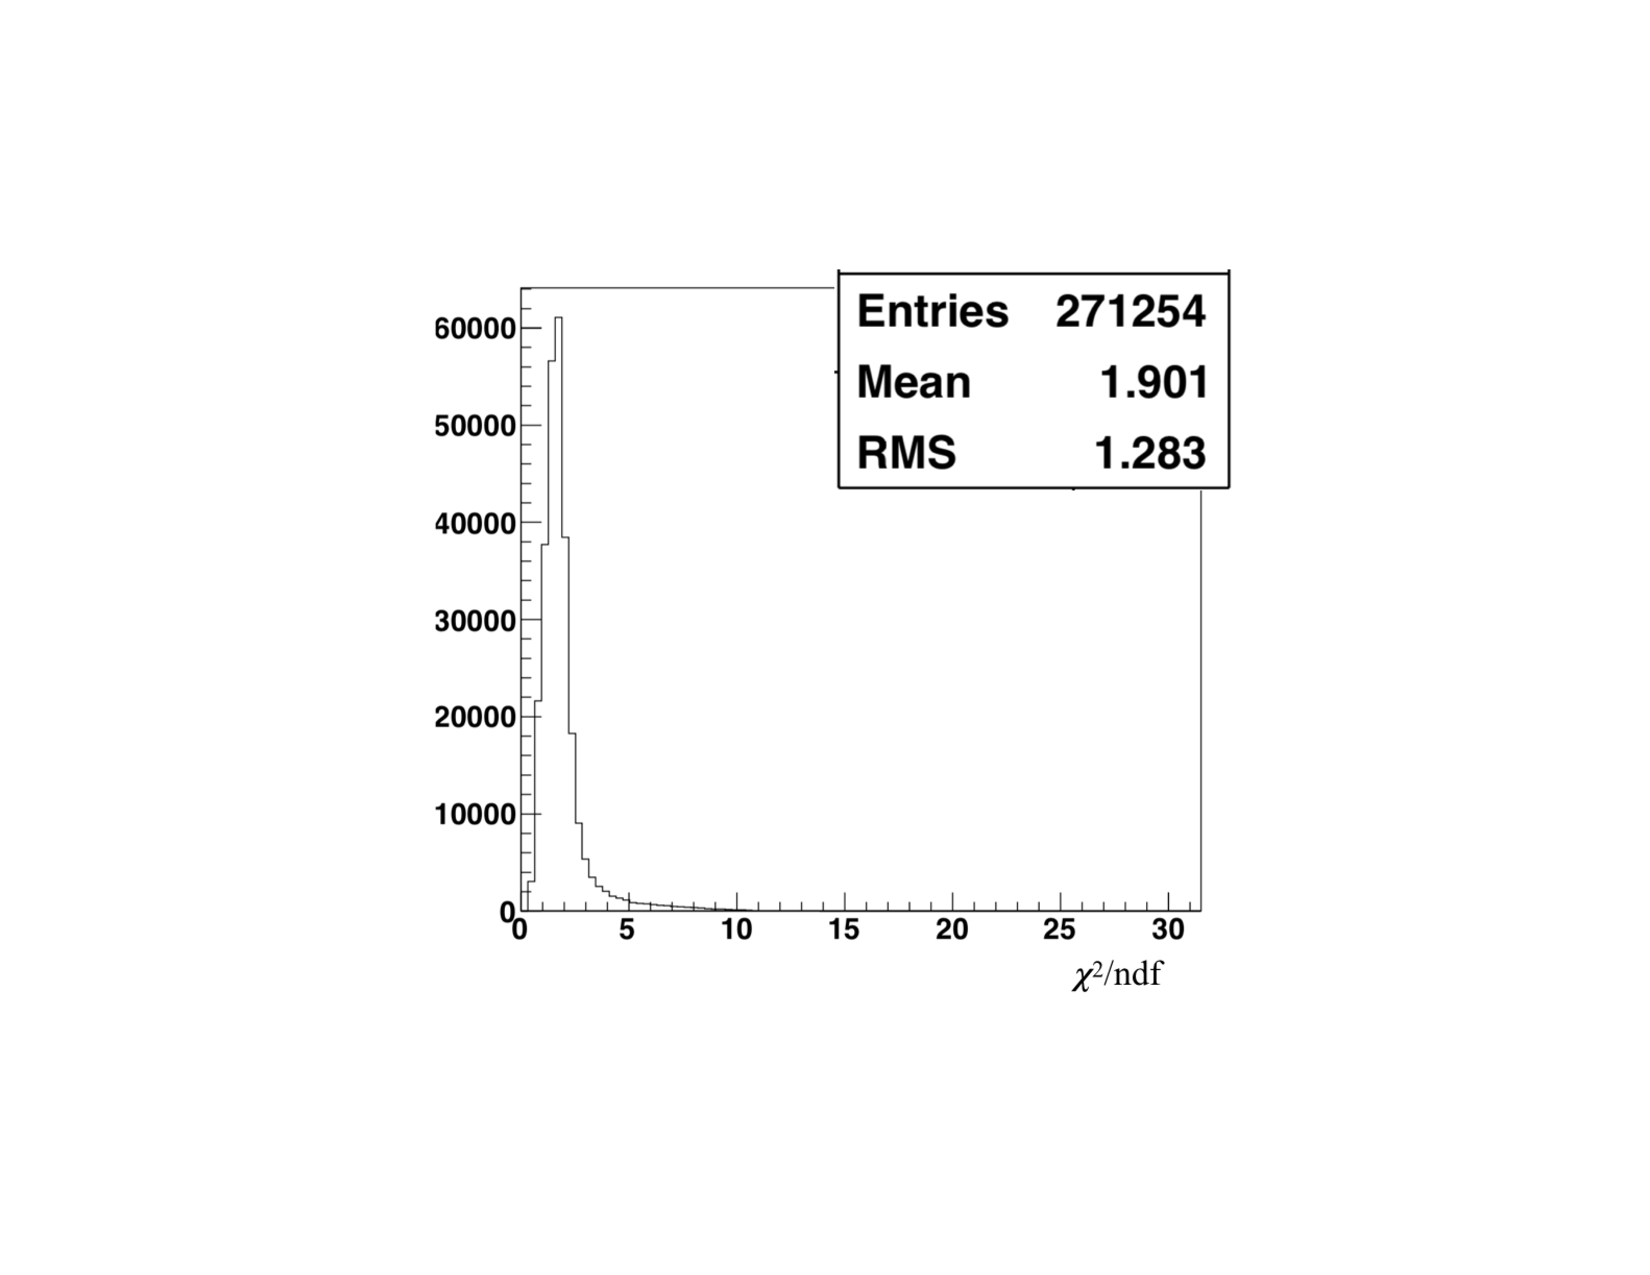
\includegraphics[width=0.5\textwidth, trim=5cm 4.5cm 5cm 4.5cm,
      clip]{trackChi2ndf}
    \caption{The reduced $\chi^2$ from alignment data tracks}
    \label{fig::trackChi2ndf}
  \end{figure}
  
\item The global number of tracks reconstructed.  Better alignment
  implies that more detectors can be associated with a track and therefore more
  tracks will be reconstructed.
\end{enumerate}
